\documentclass{report}
\usepackage{float}

% for the image in the title
\usepackage{tikz}

% custom spacing
\usepackage{setspace}
\onehalfspacing

% footer and header
\usepackage{fancyhdr}
% \setlength{\headheight}{15.2pt}

% underlining
\usepackage{ulem}


% Table of contents link to corresponding sections
\usepackage{hyperref}
\hypersetup{
	colorlinks,
	citecolor=black,
	filecolor=black,
	linkcolor=black,
	urlcolor=black
}

\usepackage{amsmath}
% Remove che "Chapter" string before chapters
\iffalse
\makeatletter
\def\@makechapterhead#1{%
	\vspace*{50\p@}%
	{\parindent \z@ \raggedright \normalfont
		\interlinepenalty\@M
		\Huge\bfseries  \thechapter.\quad #1\par\nobreak
		\vskip 40\p@
}}
\makeatother
\fi

% Fancy chapters
\usepackage[Bjarne]{fncychap}
% options: Sonny, Lenny, Glenn, Conny, Rejne, Bjarne, Bjornstrup

\begin{document}
	
	
	%title page
	\begin{titlepage}
		\begin{figure}[t]
			\centering
\includegraphics[width=0.3\textwidth]{images/unitn-logo}
		\end{figure}
		\begin{center}
			\textsc{ \LARGE{Università degli Studi di Trento \\}}
			\textsc{ \LARGE{Facoltà di Informatica\\ }}
			\textnormal{ \LARGE{Corso di Ingegneria del Software\\}}
			\vspace{30mm}
			\fontsize{10mm}{7mm}\selectfont 
			\textup{Fix Mi \\ Documento di Architettura}\\
		\end{center}
		
		\vspace{25mm}
		
		\centering
		\large Gruppo G43: \\ Giovanni Santini\\ Riginel Ungureanu \\ Valerio Asaro
		
		\vspace{20mm}
		
		\centering{\large{Anno Accademico 2023/2024 \\ Trento }}
		
	\end{titlepage}
	
	
	
	
	% use header and footers
	\pagestyle{fancy}
	\fancyhead[R]{\chaptername\ \thechapter}  % header
	
	%\maketitle
	\tableofcontents
	\newpage
	
	
	
	\section{Scopo del documento}
	
	Scadenza: 27 Novembre
	
	
	
	\section{Informazioni del Documento}
	
	% table
	\begin{center} % center the table
		\centering
		\begin{tabular}{ |p{4cm}|p{4cm}|  }
			\hline
			\centering Campo & \qquad\qquad Valore \\ % I found no other way...
			\hline
			Titolo del Documento & Documento di Architettura \\
			\hline
			Titolo del Progetto & Fix Mi \\
			\hline
			Autori del Documento &
			Giovanni Santini \\ & Riginel Ungureanu \\ & Valerio Asaro \\
			\hline
			Amministratore Progetto & Riginel Ungureanu\\
			\hline
			Versione del documento & 1.0 \\
			\hline
		\end{tabular}
	\end{center}
	
	
	
\chapter{Diagramma delle Classi}

\section{Carrello}
\begin{figure}[H]
	\centering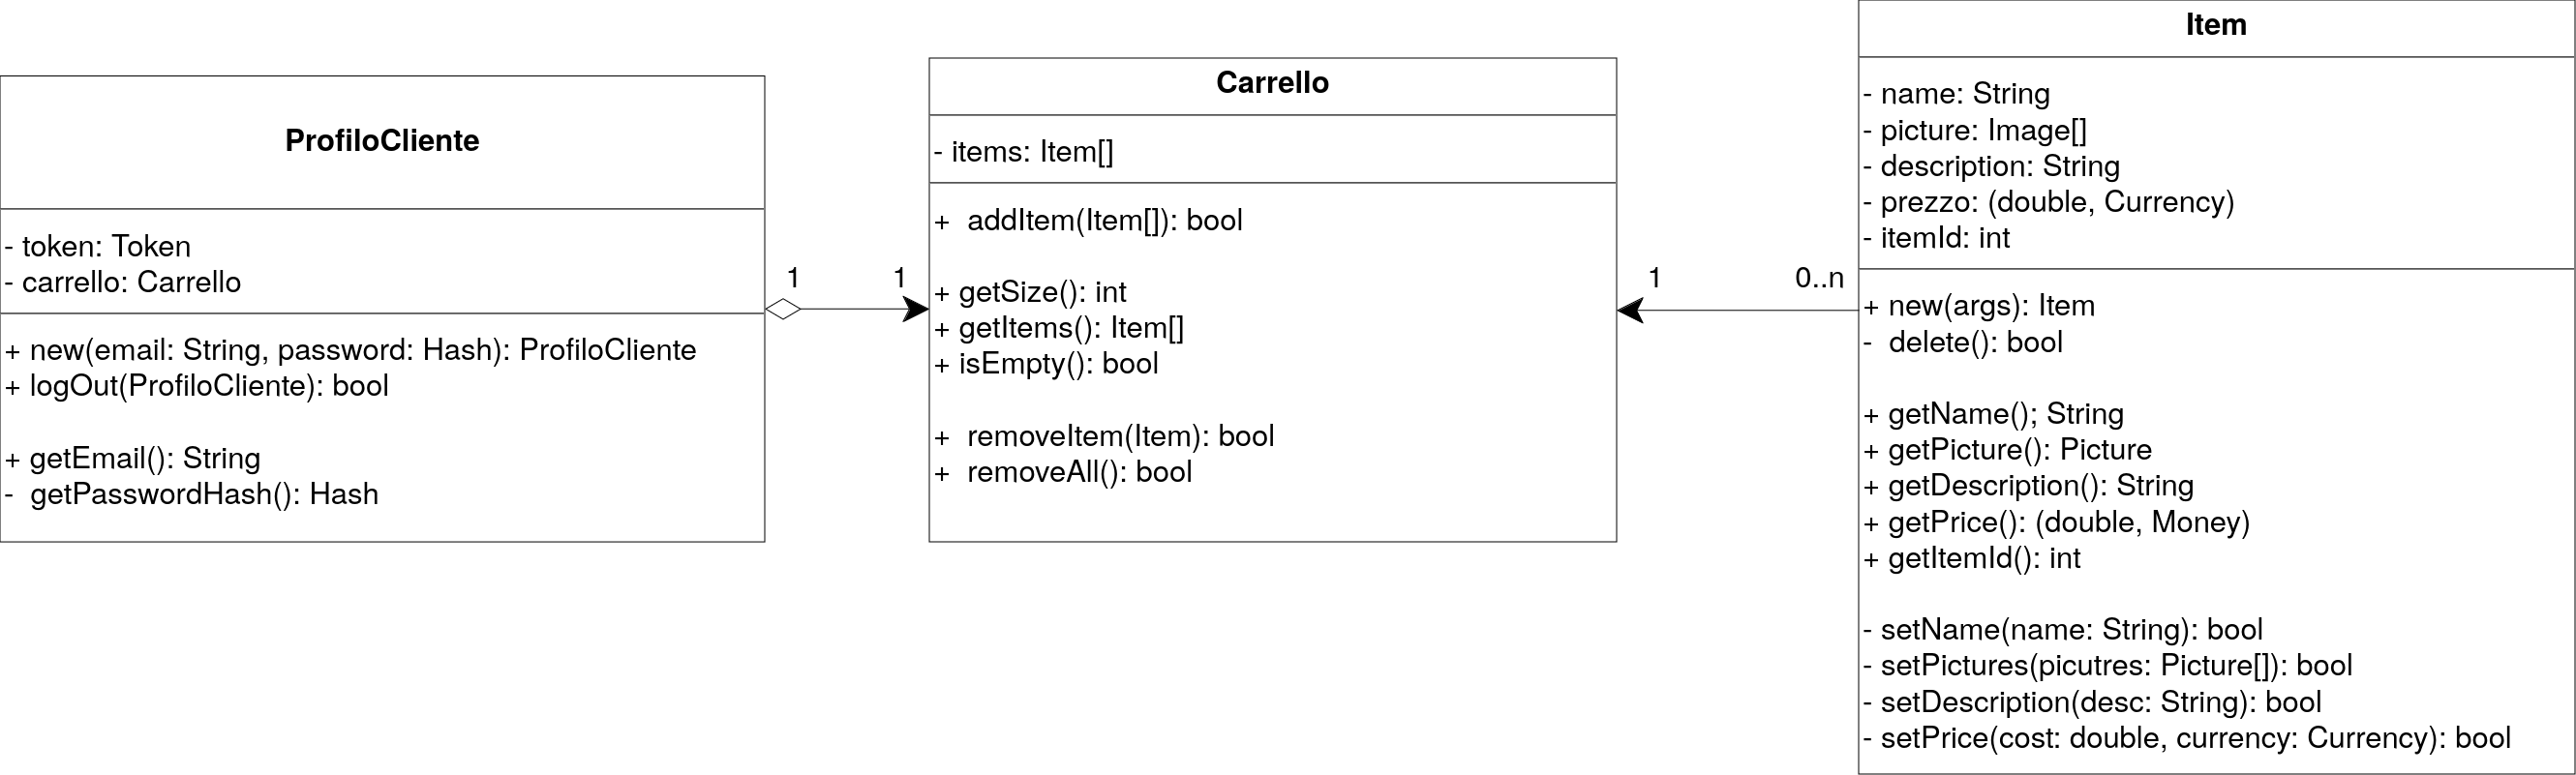
\includegraphics[width=1\textwidth]{images/Diagramma_delle_classi_carrello.png}
	Diagramma delle classi per la componente "Carrello", mostrando le classi "Carrello", "Item", "Profilo Cliente" e "Database magazzino".
\end{figure}

\subsection*{Descrizione}
Data la componente "Carrello", definita nei documenti precedenti, in riferimento ai Requisiti Funzionali numero "5.1" e "5.2", sono state individuate le classi "Carrello" e "Item". La classe Carrello contiene una lista di "Items" ed offre una serie di funzionalità come l'elencazione, l'aggiunta e la rimozione di Items dalla lista. Inoltre, ogni "Profilo Cliente", definito in precedenza, è composto anche da uno ed uno solo Carrello. A questi fini, sono stati individuati i seguenti metodi per la classe Carrello:

\begin{itemize}
\item addItem(Item[]): bool
\begin{itemize}
	\item Questo metodo permette di aggiungere uno o più Items al Database. Ritorna true se l'operazione termina con successo senza error, altrimenti ritorna flase.
\end{itemize}

\item getSize(): int
\begin{itemize}
	\item Questo metodo ritorna il numero di Items presenti nel carrello.
\end{itemize}

\item getItems(): Item[]
\begin{itemize}
	\item Questo metodo ritorna la lista di Item presente nel carrello.
\end{itemize}

\item isEmpty(): bool
\begin{itemize}
	\item Questo metodo ritorna true se non ci sono elementi nel carrello, altrimenti ritorna false.
\end{itemize}

\item removeItem(Item): bool
\begin{itemize}
	\item Dato un Item come parametro, questo metodo rimuove lo stesso dalla lista degli Items nel carrello, ritornando il risultato dell'operazione.
\end{itemize}

\item removeAll(): bool
\begin{itemize}
	\item Questo metodo rimuove tutti gli elementi dal carrello.
\end{itemize}


\end{itemize}


\subsection*{Item}
Un Item è un'oggetto presente nel magazzino, che può essere acquistato. Sono stati individuati i seguenti metodi e attributi:

\begin{itemize}

\item name: String
\begin{itemize}
	\item Il nome dell'Item.
\end{itemize}

\item picture: Image[]
\begin{itemize}
	\item Una lista di immagini associate all'Item.
\end{itemize}

\item description: String
\begin{itemize}
	\item Una descrizione dell'Item
\end{itemize}

\item prezzo: (double, Currency)
\begin{itemize}
	\item Il prezzo, salvato come una coppia di un numero reale (double) e una Currency
\end{itemize}

\item  itemId: int
\begin{itemize}
	\item Un numero identificativo ed univoco dell'Item
\end{itemize}

\item  new(args): Item
\begin{itemize}
	\item Questo metodo svolge la funzione di costruttore dell'Item, gli attributi vengono passati come argomenti alla funzione stessa. Ritorna un nuovo oggetto Item con i alori passati.
\end{itemize}

\item  delete(): bool
\begin{itemize}
	\item Questo metodo permette di eliminare l'istanza dell'oggetto Item.
\end{itemize}

\end{itemize}

Segue un'elencazione di metodi getter e setter degli attributi specificati sopra:
\begin{itemize}
\item  getName(); String

\item getPicture(): Picture

\item getDescription(): String

\item getPrice(): (double, Money)

\item getItemId(): int

\item setName(name: String): bool

\item setPictures(picutres: Picture[]): bool

\item setDescription(desc: String): bool

\item setPrice(cost: double, currency: Currency): bool

\end{itemize}

\subsection*{ProfiloCliente}

Ogni profilo cliente è composto da uno e uno solo carrello, inizialmente inizializzato con una lista vuota di Items. Il Cliente potrà accedere ed interagire con il proprio carrello nella pagina negozio speficata successivamente.



\section{Negozio}


\begin{figure}[H]
	\centering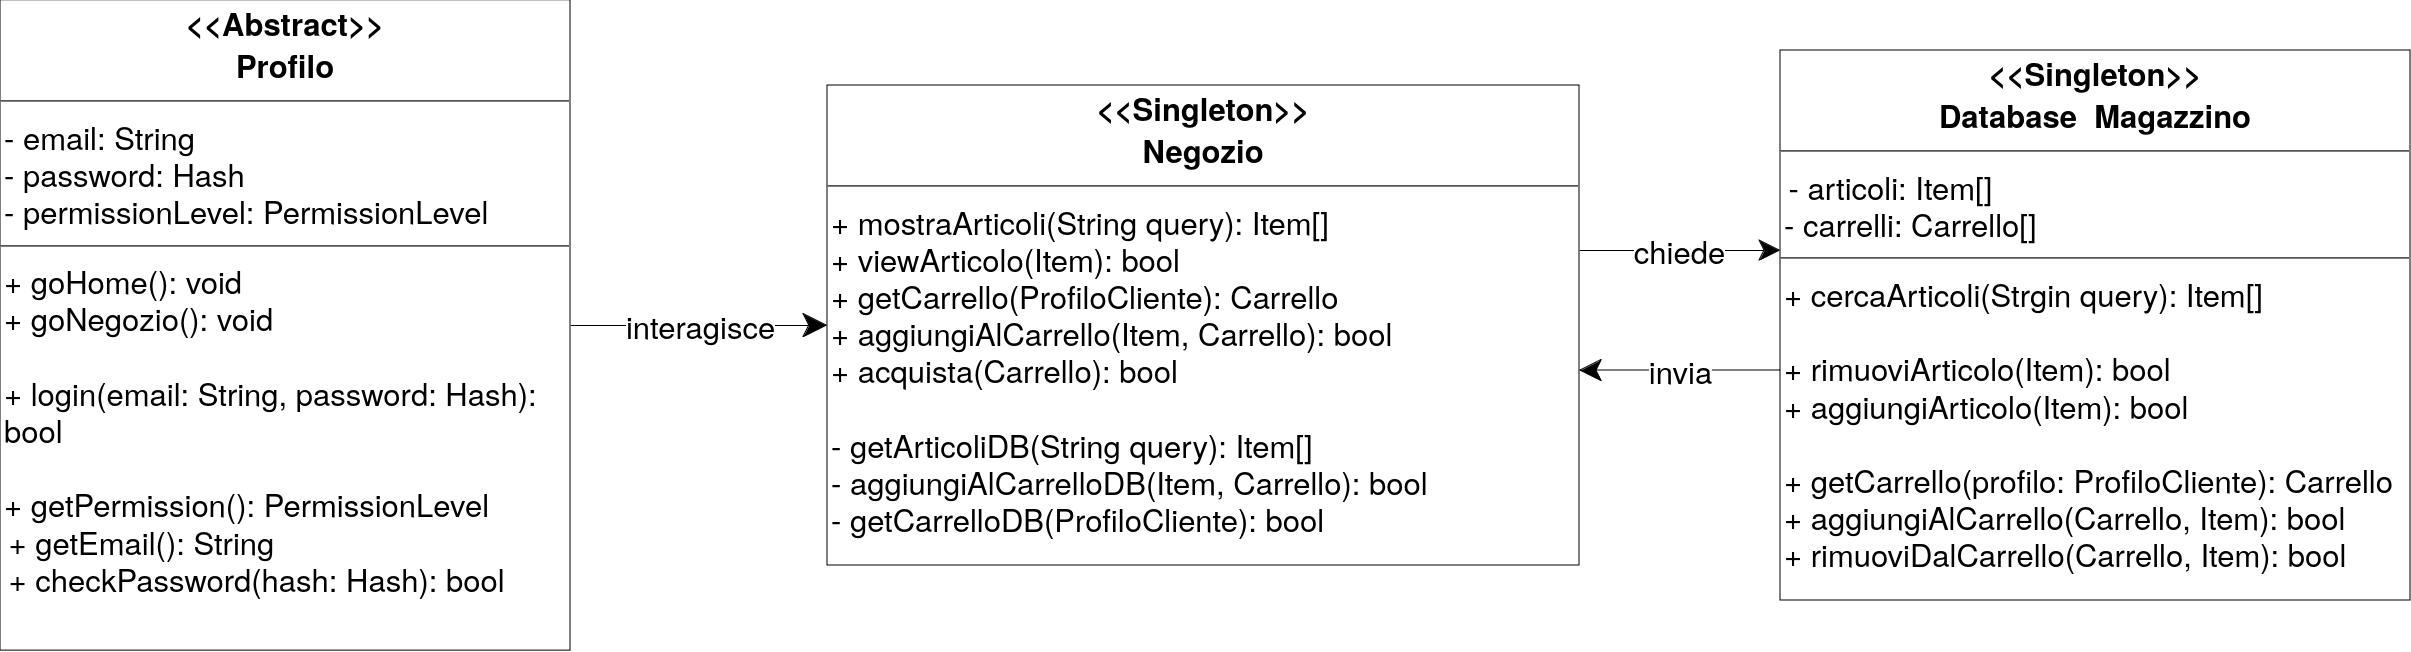
\includegraphics[width=1\textwidth]{images/Diagramma_delle_classi_negozio_2.png}
	Diagramma delle classi per la componente "Negozio" in relazione alle classi "Database Magazzino" e "Profilo"
\end{figure}

\subsection*{Descrizione}

Data la componente "Negozio", definita nel diagramma delle componenti, è stata individuata la classe "Negozio". Tale classe si pone come tramite tra l'utente e il Database Magazzino, dando la possibilità di visionare gli articoli presenti nel magazzino e, qualora l'utente fosse autenticato, di aggiungere / rimuovere articoli dal carrello. A tali fini, in riferimento alla componente "Negozio" citata sopra, vengono fortini  i seguenti metodi pubblici:

\begin{itemize}

\item mostraArticoli(String query): Item[]
\begin{itemize}
	\item Questo metodo ritorna una lista di Item data una query al DB. 
\end{itemize}

\item viewArticolo(Item): bool
\begin{itemize}
	\item Questo metodo permette di visualizzare le informazioni relative ad un'articolo nella pagina del negozio. Ritorna true se l'operazione avviene con successo, altrimenti false.
\end{itemize}


\item getCarrello(ProfiloCliente): Carrello
\begin{itemize}
	\item Dato un ProfiloCliente, questo metodo ritorna il carrello associato al profilo.
\end{itemize}


\item aggiungiAlCarrello(Item, Carrello): bool
\begin{itemize}
	\item Questo metodo permette di aggiungere un item al carrello, dati questi elementi, interfacciandosi al databse. Ritorna true se il procedimento è andato a buon fine, false altrimenti.
\end{itemize}


\item acquista(Carrello): bool
\begin{itemize}
	\item Questo metodo permette di acquistare gli item inseriti nel carrello. Ritorna true se il procedimento è andato a buon fine, false altrimenti.
\end{itemize}

\end{itemize}

Questi metodi si interfacciano alla classe Database Magazzino utilizzando i seguenti metodi privati:
\begin{itemize}
	\item getArticoliDB(String query): Item[]
	\item aggiungiAlCarrelloDB(Item, Carrello): bool
	\item getCarrelloDB(ProfiloCliente): bool
\end{itemize}

\subsection*{Database Magazzino}

La classe Datamase Magazzino ha il compito di interfacciarsi direttamente con il Database per salvare in modo persistente gli articoli e i carrelli. la classe presenta dei metodi pubblici per interagire con la base di dati come setters e getters. 

In particolare sono stati individuati i seguenti metodi:


\begin{itemize}
	\item cercaArticoli(Strgin query): Item[]
	\begin{itemize}
		\item Questo metodo permette di interrogare il database tramite una query, ritornando il risultato dell'interrogazione. 
	\end{itemize}
	\item rimuoviArticolo(Item): bool
	\begin{itemize}
		\item Questo metodo permette di rimuovere un'articolo dal database. Ritorna true solo se l'operazione è terminata con successo, false altrimenti.
	\end{itemize}
	\item aggiungiArticolo(Item): bool
	\begin{itemize}
		\item Questo metodo permette di aggiungere un'articolo ad database. Ritorna true solo se l'operazione è terminata con successo, altrimenti false.
	\end{itemize}
	\item getCarrello(profilo: ProfiloCliente): Carrello
	\begin{itemize}
		\item Questo metodo ritorna il carrello associato ad un ProfiloCliente.
	\end{itemize}
	\item aggiungiCarrello(Carrello, Item): bool
	\begin{itemize}
		\item Questo metodo permette di aggiungere un item al carrello. Richiede come parametri questi stessi e ritorna true se l'operazione è avvenuta con successo, altrimenti false.
	\end{itemize}
	
\end{itemize}

\subsection*{Profilo}
Ogni utente è in grado di accedere al Negozio, dunque è stato individuato il metodo "goNegozio()" che permetterà all'utente anche non autenticato di accedere alla pagina Negozio.

Il seguente diagramma riassume quanto detto precedentemente riguardo le classi Negozio, Database Magazzino, Profilo Cliente, Carrello, Item.


\begin{figure}[H]
	\centering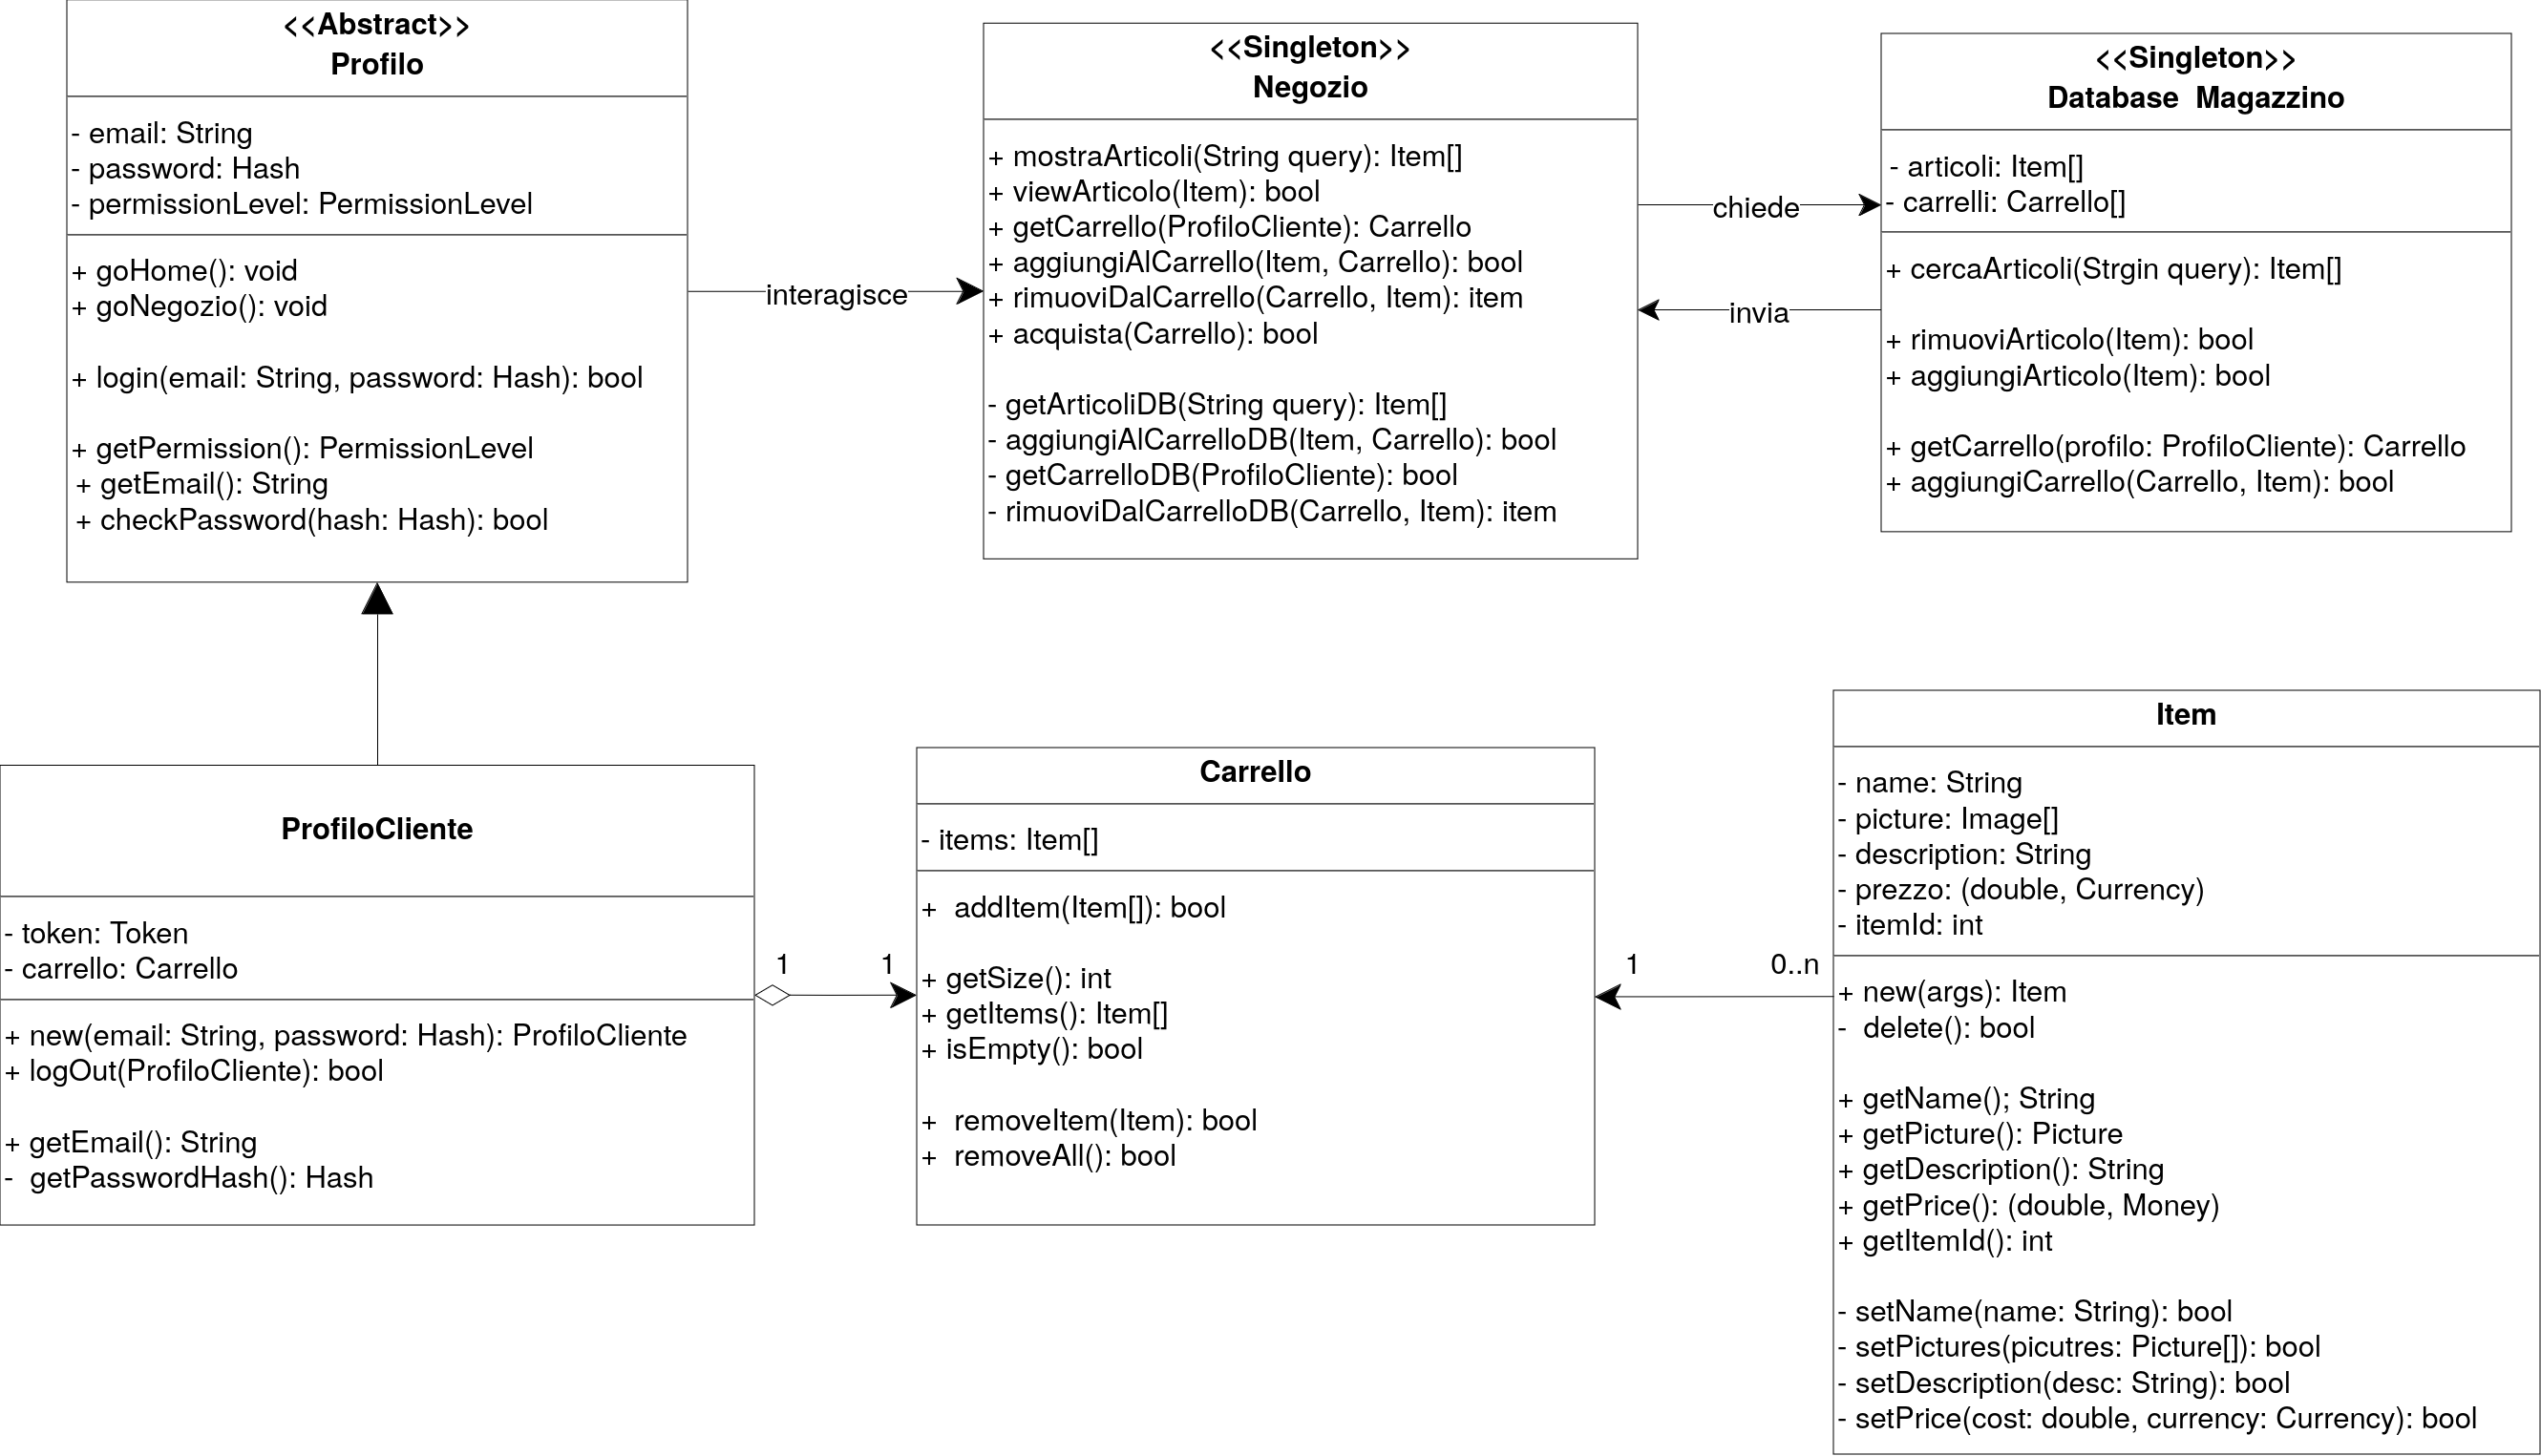
\includegraphics[width=1\textwidth]{images/Diagramma_delle_classi_negozio_1.png}
	Diagramma delle classi per la componente "Negozio" in relazione alle classi "Database Magazzino" e "Profilo Cliente"
\end{figure}



\section{Magazzino}

\begin{figure}[H]
	\centering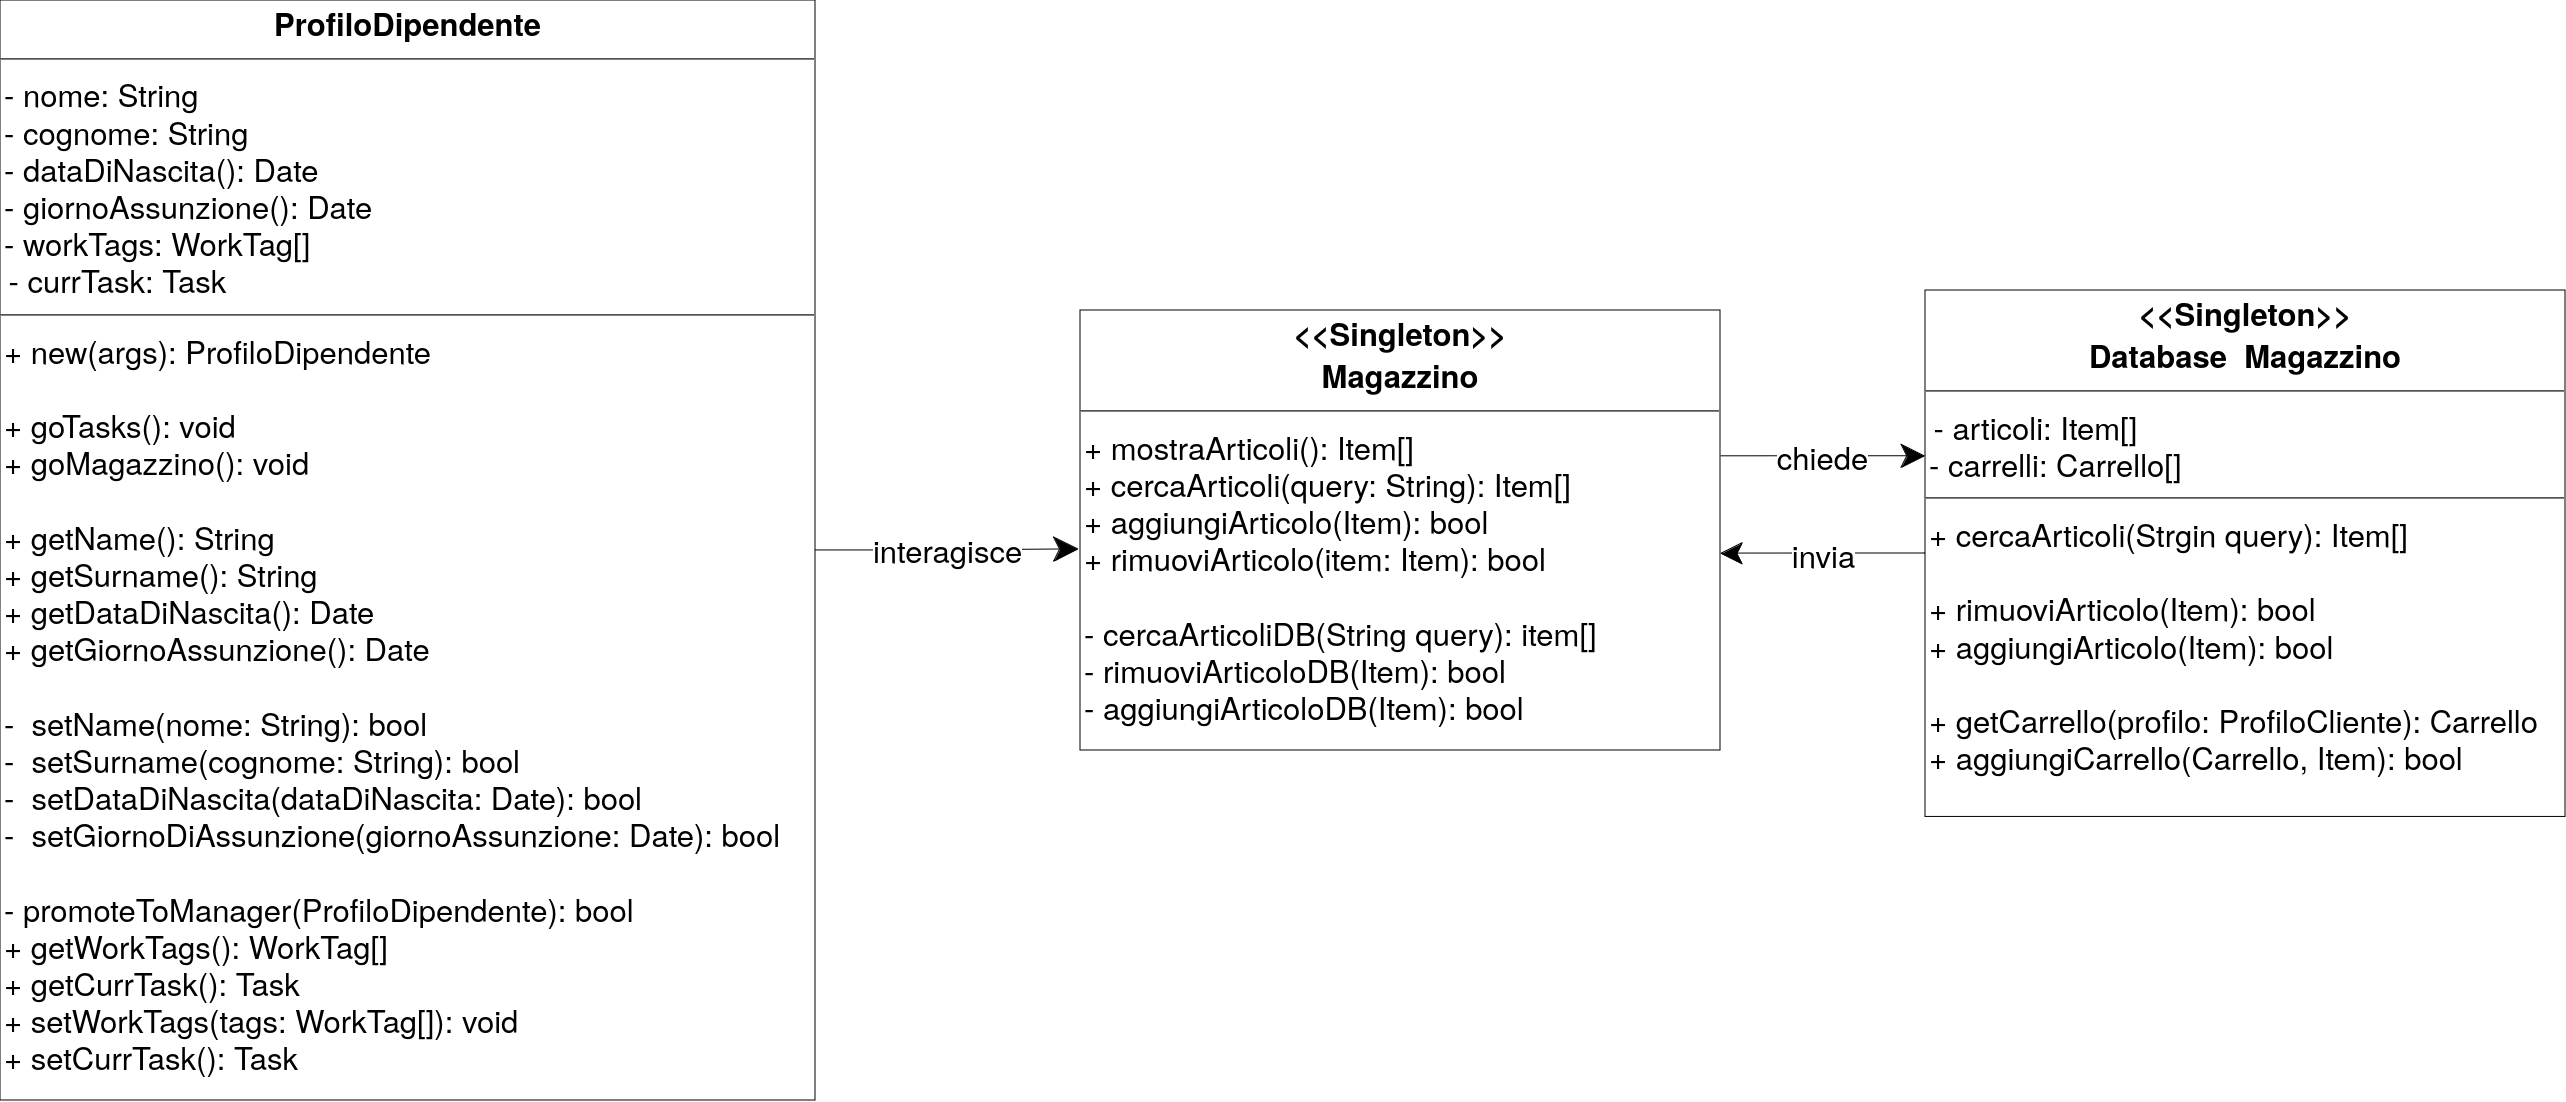
\includegraphics[width=1\textwidth]{images/Diagramma_delle_classi_magazzino.png}
	Diagramma delle classi per la componente "Magazzino", mostrando le classi "Magazzino", "ProfiloDipendente" e "Database Magazzino".
\end{figure}

\subsection*{Descrizione}
Data la componente Magazzino, secondo quanto definito in Requisito Funzionale numero "10", viene individuata la classe Magazzino. Tale classe è composta da una pagina Magazzino e permette al dipendente di interagire con il Database Magazzino, aggiungendo e rimuovendo Articoli dall stesso e dando la possibilità di cercare tali articoli attraverso interrogazioni al database. 

Vengono definiti i seguenti metodi:


\begin{itemize}
\item mostraArticoli(): Item[]
\begin{itemize}
	\item Questo metodo ritorna tutti gli articoli presenti nel Database Magazzino.
\end{itemize}

\item cercaArticoli(query: String): Item[]
\begin{itemize}
	\item Questo metodo permette di interrogate il Database Magazzino passando come argomento una stringa "query" che contiene la richiesta.
\end{itemize}

\item aggiungiArticolo(Item): bool
\begin{itemize}
	\item Questo metodo permette di aggiungere un oggetto Item al Database Magazzino.
\end{itemize}

\item rimuoviArticolo(Item): bool
\begin{itemize}
	\item Questo metodo permette al dipendente di rimuovere un oggetto Item dal Database Magazzino.
\end{itemize}

\end{itemize}

La classe Magazzino interagisce con il Database Magazzino attraverso i metodi:

\begin{itemize}
\item cercaArticoliDB(String query): item[]
\item rimuoviArticoloDB(Item): bool
\item aggiungiArticoloDB(Item): bool
\end{itemize}


\subsection*{ProfiloDipendente}

Il profilo dipendnte è in grado di raggiungere la pagina magazzino attraverso il metodo "goMagazzino()".

\subsection*{Database Magazzino}

La classe magazzino interagisce direttamente con la classe Database Magazzino che garantisce la persistenza dei dati.


\chapter{Codice in Object Constraint Language}	
	
\chapter{Diagramma delle classi con codice OCL}
	
\end{document}